\textbf{Low Rank Adaptation (LoRA)} \cite{hu2021lora} is another PEFT method for fine tuning LLMs. Main principle behind LoRA is fixing the weights of the original model and then injecting trainable low rank decomposition matrix into the current LLM architecture. 

\begin{enumerate}
    \item \textbf{Architecture of the LoRA}

    Architecture of model is modified in following way. The original weights $W_{0}$ are fixed and additional trainable weights $\Delta W$ are introduced. $\Delta W$ can be decomposed to $BA$, where rank of both matrices $B$ and $A$ is much smaller than rank of the original $W_{0}$. Resulting weights are constructed as composition $W_{0} + \Delta W = W_{0} + BA$. This way much lower number of parameters is needed to be trained. Graphical depiction can be seen in Figure ~\ref{fig:LoRA}.

    \begin{figure}[h!]
        \centering
        {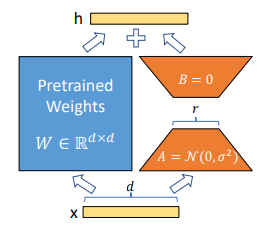
\includegraphics[scale=0.9]{imgs/LoRA.png}}
        \caption{schematic architecture of LoRa \cite{hu2021lora}}
        \label{fig:LoRA}
    \end{figure}
    
    \item \textbf{Empirical results}
    
    It turns out that LoRA performs similarly or even outperforms other methods compared in the paper, while having comparable or lower number of trainable parameters.
    For example comparing full finetuning of GPT-3 model with LoRA finetuning of the same model, the number of trainable parameters was reduced 10000 times and GPU memory requirement was reduced 3 times.
    
    Authors of the paper also noted that surprisingly low rank (as low as 1) is already yielding good results.
    
    \item \textbf{LoRA benefits}
    
    \begin{itemize}
        \item having relatively small amount of parameters to train
        \item not introducing additional latency, unlike e.g. adapter methods
        \item being able to deploy several specialized models at once, as LoRA reduces memory and computational footprint. LoRA does this by having several trained decomposition matrices for each specialized task while keeping the weights for the base model fixed.
    \end{itemize}
\end{enumerate}
